%%%%%%%%%%%%%%%%%%%%%%%%%%%%%%%%%%%%%%%%%%%%%%%%%%%%%%%%%%%%%%%%%%%%%%
% BAB METODOLOGI (Revisi Total)
%=====================================================================
\renewcommand{\thechapter}{\Roman{chapter}}
\addtocontents{toc}{\vskip10pt}
\chapter{METODOLOGI PENELITIAN}
\renewcommand{\thechapter}{\arabic{chapter}}
%---------------------------------------------------------------------

Penelitian ini menggunakan pendekatan komputasi multi-skala untuk menyelidiki pengaruh temperatur dan defek titik terhadap sifat elektronik dan magnetik monolayer hBN.
Alur kerja penelitian dibagi menjadi dua tahap utama: (1) generasi struktur atomik yang setimbang secara termal menggunakan simulasi Dinamika Molekuler (MD) klasik, dan (2) perhitungan sifat elektronik dan magnetik dari prinsip pertama menggunakan Teori Fungsional Kerapatan (DFT) pada struktur yang dihasilkan.
\section{Perangkat Penelitian}
\subsection{Perangkat Keras}
Seluruh simulasi komputasi dilakukan pada klaster komputasi performa tinggi dengan spesifikasi sebagai berikut:
\begin{itemize}
    \item 3 node komputasi, masing-masing dengan 1x CPU AMD EPYC 7702P (64 core/128 thread, 2.0 GHz).
\item Memori RAM 240 GB per node.
    \item Interkoneksi antar node menggunakan Mellanox RoCE 100Gbps.
\end{itemize}

\subsection{Perangkat Lunak}
Perangkat lunak yang digunakan dalam penelitian ini meliputi:
\begin{itemize}
    \item \textbf{LAMMPS (\textit{Large-scale Atomic/Molecular Massively Parallel Simulator}):} Digunakan untuk simulasi MD \citep{Plimpton1995}.
\item \textbf{Quantum ESPRESSO:} Digunakan untuk perhitungan DFT dari prinsip pertama \citep{Giannozzi2009, Giannozzi2017}.
\item \textbf{Atomic Simulation Environment (ASE):} Digunakan untuk pembuatan model struktur dan konversi format file antar perangkat lunak.
\item \textbf{VMD, OVITO, XCrySDen, VESTA:} Digunakan untuk visualisasi struktur atomik, kerapatan muatan, dan kerapatan spin.
\item \textbf{Python (NumPy, Matplotlib):} Digunakan untuk analisis data dan pembuatan plot hasil komputasi.
\end{itemize}

\begin{figure}[htbp]
    \centering

    \begin{subfigure}{0.8\linewidth}
        \centering
        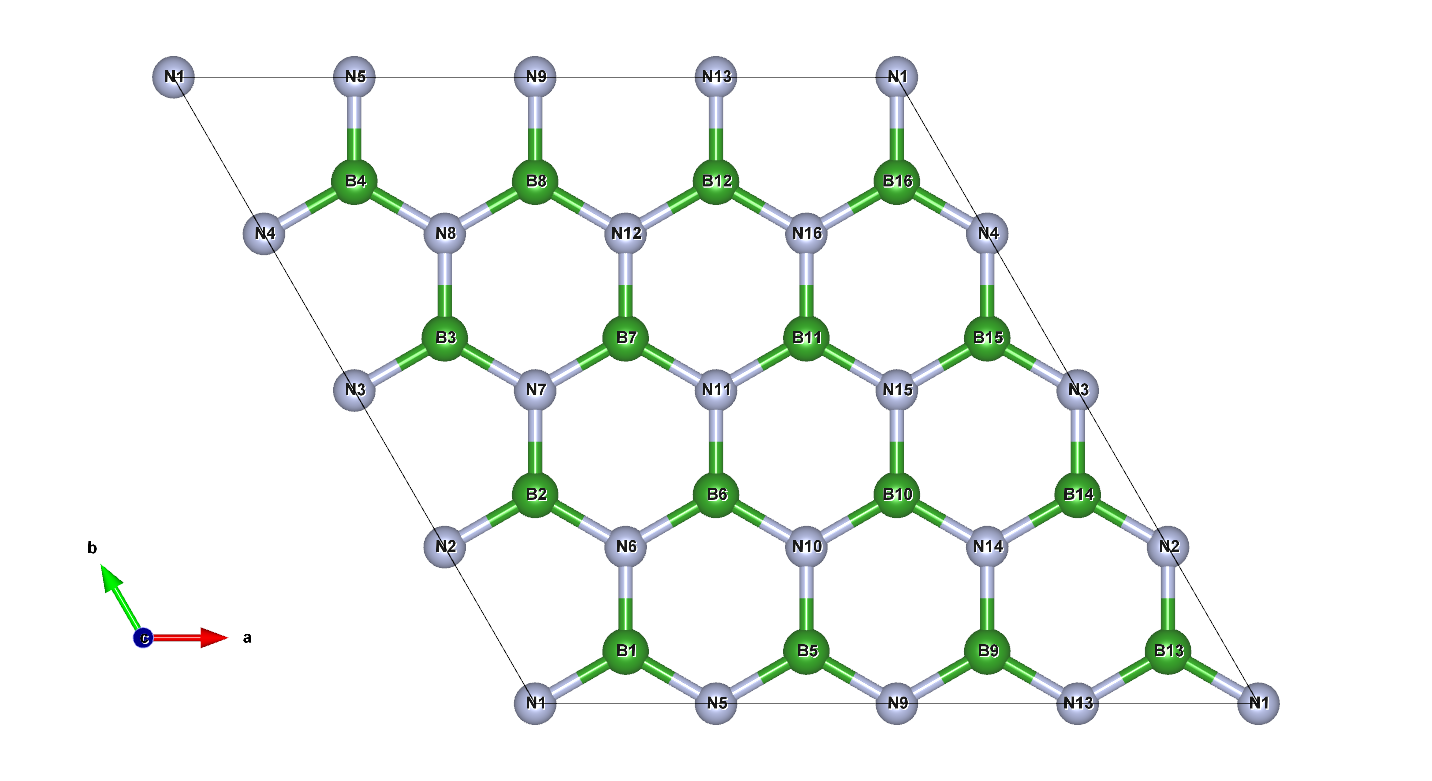
\includegraphics[width=\linewidth]{gambar_hasil/pure_hBN_4x4x1.png}
        \caption{Struktur hBN murni}
    \end{subfigure}
    \vspace{0.5cm} % jarak antar gambar

    \begin{subfigure}{0.8\linewidth}
        \centering
        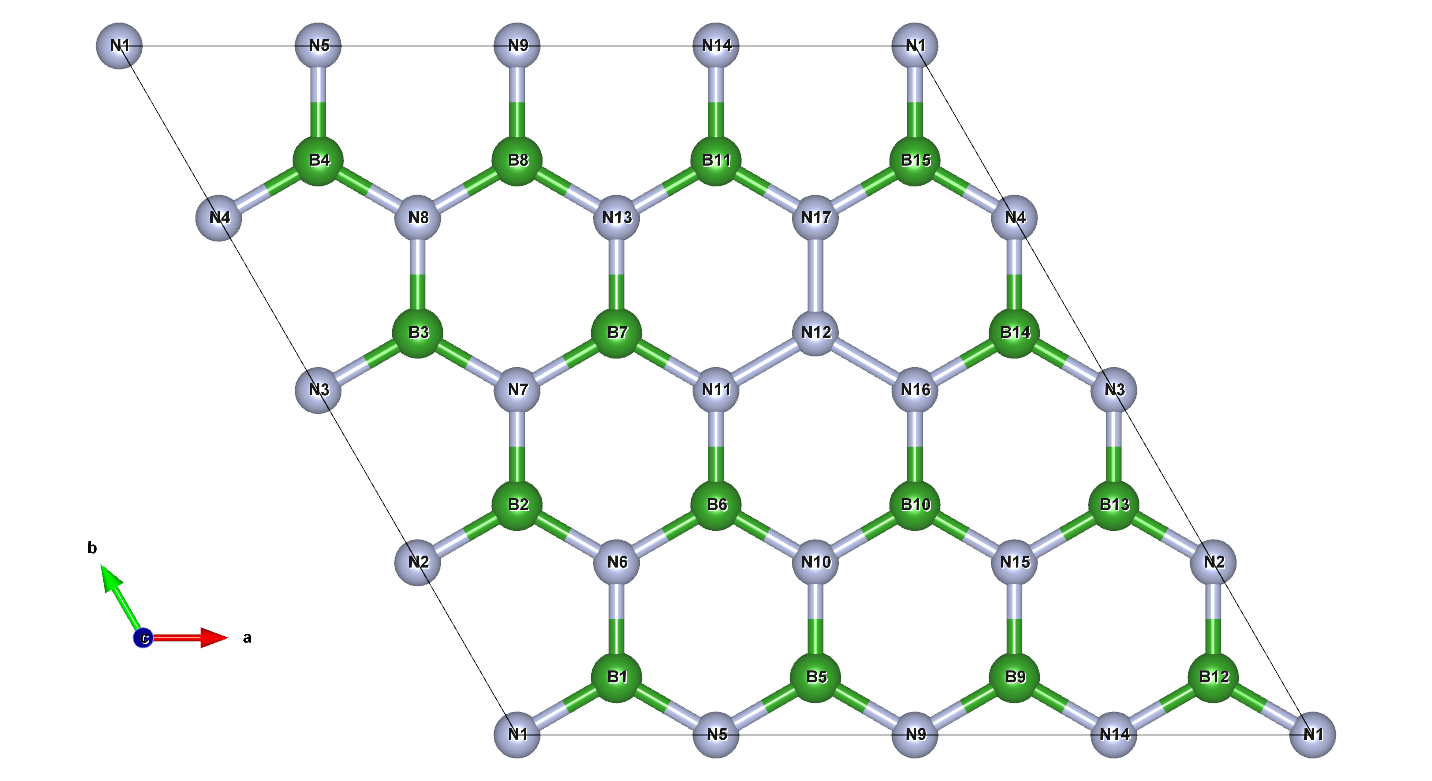
\includegraphics[width=\linewidth]{gambar_hasil/NN_defect_hBN_center_4x4x1.png}
        \caption{Struktur hBN dengan cacat N-N}
    \end{subfigure}
    \vspace{0.5cm}

    \begin{subfigure}{0.8\linewidth}
        \centering
  
      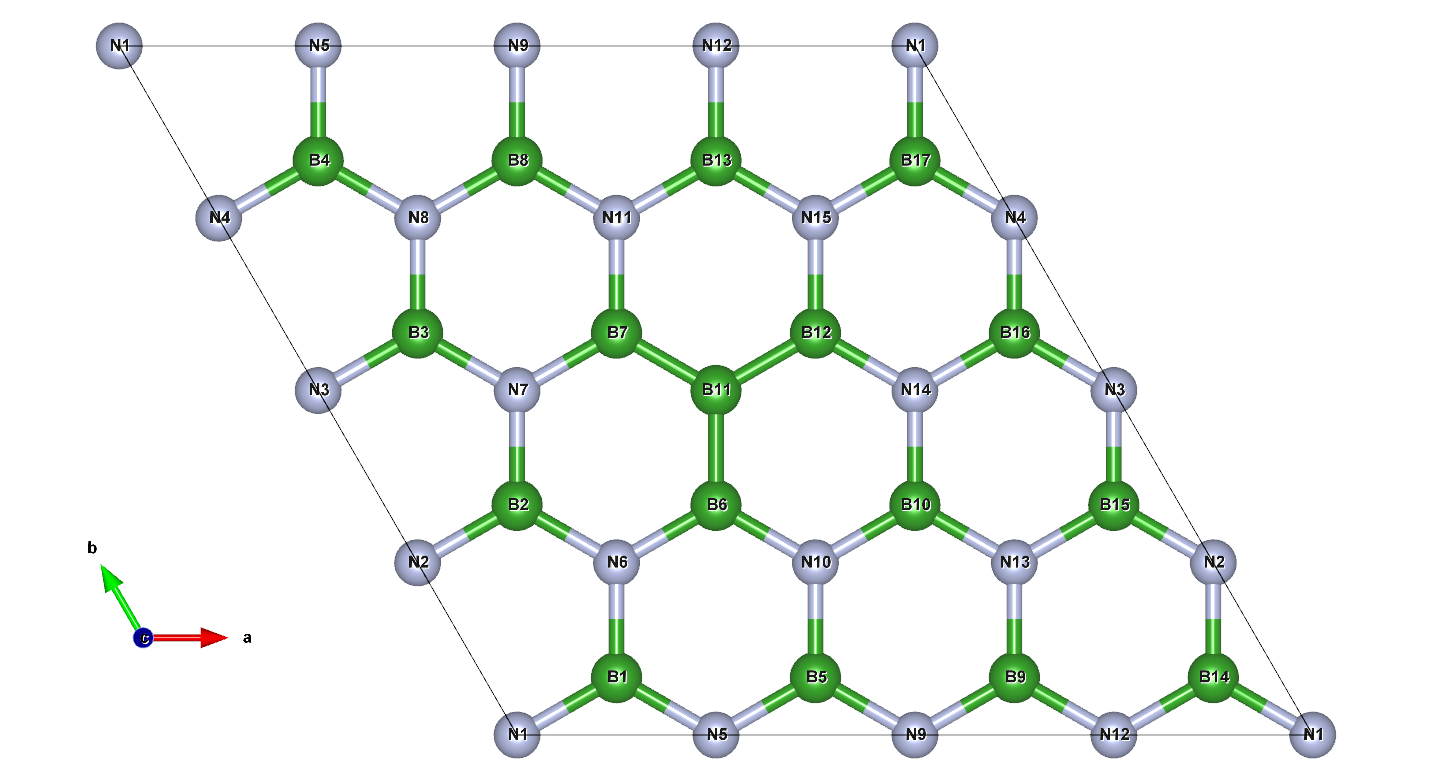
\includegraphics[width=\linewidth]{gambar_hasil/BB_defect_hBN_center_4x4x1.png}
        \caption{Struktur hBN dengan cacat B-B}
    \end{subfigure}

    \caption{Model hBN 4$\times$4$\times$1 dengan berbagai konfigurasi cacat}
    \label{fig:struktur_hBN_4x4x1}
\end{figure}

\section{Prosedur Penelitian}

\subsection{Tahap 1: Generasi Struktur Termal dengan Dinamika Molekuler}
Tujuan dari tahap ini adalah untuk mendapatkan konfigurasi atomik yang realistis dari monolayer hBN pada temperatur tinggi, yang menangkap efek vibrasi termal dan relaksasi struktural lokal.
\subsubsection{Model Sistem Komputasi}
Tiga jenis sistem dimodelkan menggunakan supercell monolayer hBN berukuran $4 \times 4 \times 1$, yang terdiri dari 32 atom (16 atom B dan 16 atom N).
Ruang vakum setebal 20 Å ditambahkan pada arah-z untuk mencegah interaksi antar citra periodik.
Sistem-sistem tersebut adalah:
\begin{enumerate}
    \item \textbf{hBN Murni (\textit{Pristine}):} Supercell hBN ideal tanpa defek.
\item \textbf{hBN dengan Defek N$_B$:} Satu atom Boron digantikan oleh satu atom Nitrogen.
\item \textbf{hBN dengan Defek B$_N$:} Satu atom Nitrogen digantikan oleh satu atom Boron.
\end{enumerate}
Visualisasi model-model ini dapat dilihat pada Gambar \ref{fig:struktur_hBN_4x4x1}.

\begin{figure}
    \centering
    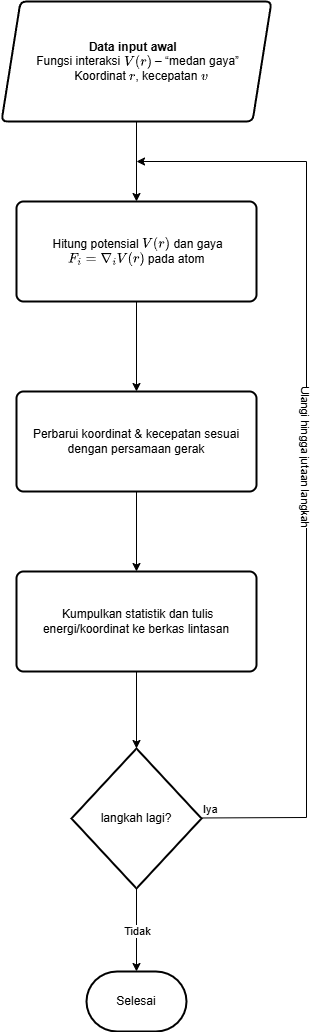
\includegraphics[width=0.6\linewidth]{gambar/MD.drawio.png}
    \caption{Alur Komputasi MD}
    \label{Diagram Alir MD}
\end{figure}

\begin{figure}
    \centering
    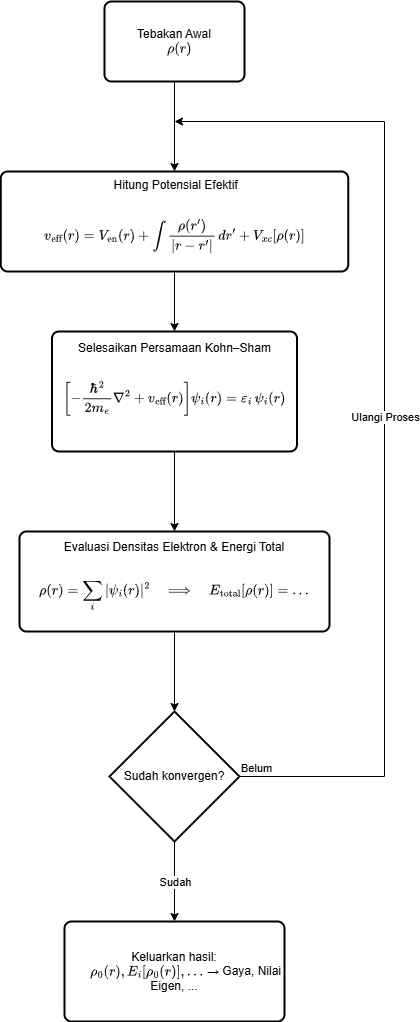
\includegraphics[width=0.6\linewidth]{gambar/DFT.drawio.png}
    \caption{Alur Komputasi DFT }
    \label{Diagram Alir DFT}
\end{figure}



\subsubsection{Detail Simulasi MD}
Simulasi MD dilakukan menggunakan perangkat lunak LAMMPS.
\begin{itemize}
    \item \textbf{Potensial Interatomik:} Interaksi antar atom dimodelkan menggunakan potensial ReaxFF yang diparameterisasi oleh Lele et al.
\citep{Lele2022}. Perlu dicatat bahwa potensial ini secara spesifik dikembangkan untuk memodelkan sintesis fasa gas dan mekanisme reaksi.
Penggunaannya untuk mensimulasikan dinamika termal fasa padat, seperti dalam penelitian ini, membawa asumsi bahwa potensial ini cukup akurat dalam mendeskripsikan vibrasi kisi dan relaksasi struktural.
Validitas asumsi ini akan dievaluasi secara kritis pada Bab IV.
\item \textbf{Prosedur Simulasi:}
    \begin{enumerate}
        \item \textbf{Relaksasi Awal:} Setiap struktur awal direlaksasi energinya pada 0 K untuk meminimalkan gaya-gaya internal.
\item \textbf{Kesetimbangan Termal:} Sistem kemudian dipanaskan dan disetimbangkan pada tiga temperatur target—800K, 1100K, dan 1225K—menggunakan ensemble kanonik (NVT) dengan thermostat Nosé-Hoover.
Langkah waktu integrasi yang digunakan adalah 0.25 fs.
        \item \textbf{Ekstraksi Struktur:} Setelah sistem mencapai kesetimbangan termal pada setiap temperatur target, satu potret (snapshot) konfigurasi atomik (koordinat) diekstraksi dari lintasan MD.
Struktur statis inilah yang menjadi input untuk tahap perhitungan DFT selanjutnya.
\end{enumerate}
\end{itemize}

\subsubsection{Analisis Struktural dan Dinamis dari Trajektori MD}
\label{sec:md_analysis}
Meskipun tujuan utama dari tahap MD adalah untuk menghasilkan satu struktur representatif untuk perhitungan DFT, analisis terhadap keseluruhan trajektori MD juga dilakukan untuk memahami evolusi struktur dan dinamika atom selama proses pemanasan. Analisis ini memberikan konteks penting untuk interpretasi hasil DFT. Dua kuantitas utama yang dihitung adalah:
\begin{itemize}
    \item \textbf{Radial Distribution Function (RDF), $g(r)$:} RDF dihitung untuk mengkarakterisasi tatanan jarak dekat dalam sistem pada setiap temperatur. Fungsi ini memberikan probabilitas untuk menemukan pasangan atom pada jarak $r$. Analisis RDF untuk pasangan atom B-N, B-B, dan N-N memungkinkan pemantauan perubahan panjang ikatan, koordinasi atom, dan indikasi awal pelelehan (melting) yang ditandai dengan melebarnya puncak-puncak RDF.
    \item \textbf{Mean Squared Displacement (MSD):} MSD dihitung untuk mengukur mobilitas atom dan mengidentifikasi transisi fasa. MSD didefinisikan sebagai perpindahan kuadrat rata-rata atom dari posisi awalnya seiring waktu. Pada fasa padat, atom-atom bergetar di sekitar posisi kesetimbangannya, sehingga MSD akan mencapai nilai jenuh (plateau). Sebaliknya, pada fasa cair, atom-atom dapat berdifusi, yang tercermin dari peningkatan MSD secara linear terhadap waktu. Analisis ini digunakan untuk memvalidasi keadaan termal (padat atau cair) dari struktur pada temperatur target.
\end{itemize}

\subsection{Tahap 2: Kalkulasi Sifat Elektronik dengan Teori Fungsional Kerapatan}
Tujuan dari tahap ini adalah untuk menghitung secara akurat sifat elektronik dan magnetik dari konfigurasi atomik yang diperoleh dari tahap MD.
\subsubsection{Detail Perhitungan DFT}
Perhitungan DFT dilakukan menggunakan paket perangkat lunak Quantum ESPRESSO.
\begin{itemize}
    \item \textbf{Fungsional Tukar-Tambah-Hubungan:} Fungsional Perdew-Burke-Ernzerhof yang dioptimalkan untuk padatan (PBEsol) \citep{Perdew2008} dalam kerangka Aproksimasi Gradien Umum (GGA) digunakan.
Fungsional GGA seperti PBEsol dikenal secara sistematis meremehkan (\textit{underestimate}) nilai celah pita energi.
Oleh karena itu, analisis akan difokuskan pada tren kualitatif dan perubahan relatif, bukan pada nilai absolut celah pita.
\item \textbf{Pseudopotensial:} Metode \textit{Projector Augmented-Wave} (PAW) dari repositori JTH v1.1 digunakan untuk merepresentasikan interaksi antara elektron valensi dan inti atom \citep{Blochl1994, Kresse1999}.
\item \textbf{Parameter Komputasi:}
    \begin{itemize}
        \item Energi potong (\textit{cutoff energy}) untuk basis \textit{plane-wave} ditetapkan sebesar 60 Ry.
\item Zona Brillouin di-sampling menggunakan kisi Monkhorst-Pack $8 \times 8 \times 1$.
\item Metode smearing Marzari-Vanderbilt (\textit{cold smearing}) digunakan untuk membantu konvergensi numerik.
\item Perhitungan bersifat spin-terpolarisasi (\textit{spin-polarized}) untuk semua sistem guna memungkinkan kemunculan keadaan magnetik secara spontan.
\end{itemize}
\end{itemize}

\subsubsection{Prosedur Perhitungan}
Untuk setiap struktur yang diperoleh dari MD, serangkaian perhitungan DFT dilakukan sebagai berikut:
\begin{enumerate}
    \item \textbf{Perhitungan SCF (\textit{Self-Consistent Field}):} Dilakukan untuk mendapatkan kerapatan muatan dan energi total keadaan dasar dari sistem pada geometri atomik yang tetap (diperoleh dari MD).
\item \textbf{Perhitungan NSCF (\textit{Non-Self-Consistent Field}):} Dilakukan menggunakan kerapatan muatan yang telah konvergen dari langkah SCF.
Perhitungan ini menggunakan jejaring k-point yang lebih padat atau di sepanjang jalur simetri tinggi (misalnya, $\Gamma$-M-K-$\Gamma$) untuk menghitung nilai Eigen secara akurat.
\item \textbf{Pasca-pemrosesan:} Data dari perhitungan NSCF diproses lebih lanjut untuk menghasilkan:
    \begin{itemize}
        \item Struktur Pita Elektronik (\textit{Band Structure})
        \item Kerapatan Keadaan (\textit{Density of States}, DOS)
        \item Kerapatan Keadaan Terproyeksi (\textit{Projected Density of States}, PDOS)
        \item Visualisasi Kerapatan Muatan dan Kerapatan Spin.
\end{itemize}
\end{enumerate}
Dengan mengikuti prosedur yang terstruktur ini, penelitian ini dapat secara sistematis menghubungkan perubahan struktural yang diinduksi oleh temperatur dengan modifikasi sifat elektronik dan magnetik yang dihasilkan.